%
% ---
% id : "electrotechnique_puissance_20260429_224"
% title : "Rendement et diagramme de Sankey"
% domain : "Électrotechnique"
% subdomain : "Puissance"
% tags : ["rendement", "sankey", "moteur", "transformateur", "triphasé", "puissance", "ts"]
% difficulty : 2
% ---

\documentclass[a4paper,11pt,answers,addpoints]{exam}
% ---------------------------------------------------------
% LANGUE, ENCODAGE, FONTS
% ---------------------------------------------------------
\usepackage[utf8]{inputenc}

% ---------------------------------------------------------
% GÉOMÉTRIE ET MISE EN PAGE
% ---------------------------------------------------------
\usepackage[left=1.7cm,right=1.5cm,top=2cm,bottom=1cm]{geometry}
%\usepackage{a4wide}

% ---------------------------------------------------------
% MATHÉMATIQUES
% ---------------------------------------------------------
\usepackage{amsmath, amssymb, bm, esvect}

% Vecteurs
\newcommand{\V}{\overrightarrow}
\def\vect#1{\overrightarrow{\strut#1}}
\providecommand{\Degrees}[0]{\ensuremath{^\circ}}

% ---------------------------------------------------------
% UNITÉS ET GRANDEURS (SIunitx)
% ---------------------------------------------------------
\usepackage{siunitx}
\sisetup{output-decimal-marker={,}}
\DeclareSIUnit \var {var}
\DeclareSIUnit \VA {VA}
\DeclareSIUnit \kVA {kVA}
\DeclareSIUnit[quantity-product={}] \degree{\text{\textdegree}}

% ---------------------------------------------------------
% GRAPHIQUES : TikZ + CircuitikZ + PGFPlots
% ---------------------------------------------------------
\usepackage{tikz}
\usetikzlibrary{
	arrows.meta,
	intersections,
	decorations.pathreplacing,
	positioning
}

\usepackage[european,straightvoltages,EFvoltages]{circuitikz}

\usepackage{tkz-fct}
\usepackage{pgfplots}
\pgfplotsset{compat=1.12}

% Symbole étoile-triangle personnalisé
\newcommand{\wye}{%
	\mathbin{\tikz[x=1ex,y=1ex]{%
			\draw[line width=.1ex] (0,0)--(45:1)--++(-45:1) (45:1)--++(0,1);
	}}%
}


\usepackage{sankey}

\pgfdeclarelayer{background}
\pgfdeclarelayer{foreground}
\pgfdeclarelayer{sankeydebug}
\pgfsetlayers{background,main,foreground,sankeydebug}


% ---------------------------------------------------------
% TABLEAUX
% ---------------------------------------------------------
\usepackage{tabularx}
\usepackage{tabu}

% ---------------------------------------------------------
% HYPERLIENS
% ---------------------------------------------------------
\usepackage[colorlinks=true,
menucolor=red,
breaklinks=true,
urlcolor=blue,
linkcolor=blue]{hyperref}

% ---------------------------------------------------------
% COMMANDES PERSONNELLES
% ---------------------------------------------------------
\newcommand\nomauteur{bdminasmorgul@protonmail.com}
\newcommand\dateTe{29.04.2026}
\newcommand\brancheTe{TS}

% ---------------------------------------------------------
% STYLE DE L'EXERCICE
% ---------------------------------------------------------
\pagestyle{headandfoot}
\firstpageheadrule
\runningheadrule

\firstpageheader{\brancheTe\ (\nomauteur)}{Élève : }{(\dateTe) \thepage/\numpages}
\runningheader{\brancheTe\ (\nomauteur)}{Élève : }{(\dateTe) \thepage/\numpages}

% Compteur en bas de page
\newcommand{\totalpointtts}{%
	\begin{tikzpicture}[remember picture, overlay]
		\node[anchor=south west, inner sep=0pt, outer sep=0pt]
		at ([xshift=0.5cm,yshift=0.5cm]current page.south west)
		{\rotatebox{90}{Total des points : \numpoints}};
	\end{tikzpicture}
}

\firstpagefooter{\totalpointtts}{}{}
\runningfooter{\totalpointtts}{}{}

% Réglages exam
\printanswers
\addpoints
\pointsinmargin
\bracketedpoints

% ---------------------------------------------------------
% LISTINGS (code)
% ---------------------------------------------------------
\usepackage{xcolor}
\usepackage{listings}

\lstdefinestyle{octavestyle}{
	language=Matlab,
	basicstyle=\ttfamily\small,
	keywordstyle=\color{blue},
	commentstyle=\color{green!50!black},
	stringstyle=\color{red},
	stepnumber=1,
	frame=single,
	breaklines=true,
	breakatwhitespace=true,
	tabsize=4
}

% ---------------------------------------------------------
% DOCUMENT
% ---------------------------------------------------------
\begin{document}
	
	
	\unframedsolutions
	\pointsinmargin
	\bracketedpoints
	\section*{Préparation TS PQ CFC ELMO, IELE, PELE}
	\begin{questions}
		

\question Sur la base du diagramme de Sankey illustrant les flux énergétiques ou de puissances, répondre aux cinq situations indépendantes suivantes~:
\begin{center}
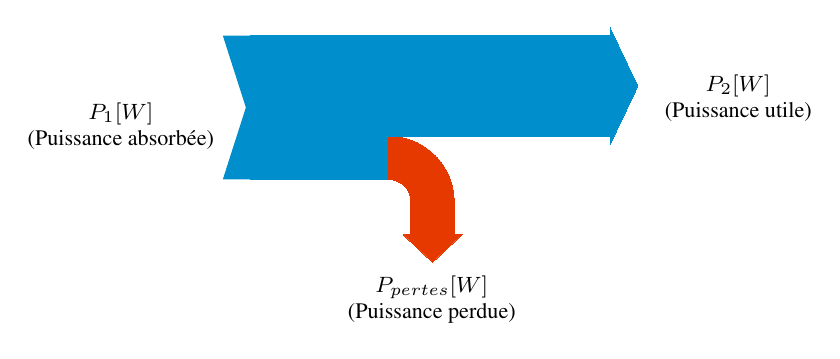
\begin{tikzpicture}
	% font choice
	\renewcommand\rmdefault{txr}\rmfamily\footnotesize
	\sisetup{
		round-mode=places,
		round-precision=1,
		add-decimal-zero,
	}
	
	\begin{sankeydiagram}
		\colorlet{energy}{blue!30!cyan!80!black}
		\colorlet{lost energy}{red!50!orange!90!black}
		\sankeyset{
			ratio=13em/100,
			minimum radius=1em,
			start style=arrow,end style=arrow,
			draw/.style={draw=none,line width=0},
			energy/.style={
				fill/.style={
					draw=energy,
					line width=0,
					fill=energy,
				}
			},
			lost energy/.style={
				fill/.style={
					draw=lost energy,
					line width=0,
					fill=lost energy,
				}
			}
		}
		\newcommand\abovelabel[2]{ % valname, label
			\node[xshift=-63pt,yshift=-44pt,anchor=south east,align=center,inner xsep=0] at (#1.left) {#2};
		}
		\newcommand\Punlabel[2]{ % valname, label
			\node[xshift=73pt,yshift=-34pt,anchor=south 		east,align=center,inner xsep=0] at (#1.left) {#2};
		}		
		\newcommand\belowlabel[2]{ % valname, label
			\node[anchor=south west,align=center,inner xsep=0, xshift=-23pt,yshift=-35pt] at 	(#1.south) {#2};
		}
		% Label de FIN (35) : inchangé
		\newcommand\energylabel[1]{ % valname
			\node[anchor=north east,text=energy,inner xsep=0] at (#1.right)
			{\num{\sankeygetnodeqty{#1}}};
		}
		
		% Label de DÉBUT (50) : corrigé avec overlay + ancre east
		\newcommand\energylabelstart[1]{ % valname
			\node[overlay, anchor=east, text=energy, inner xsep=0, yshift=-30pt, xshift=-61pt] at (#1.left)
			{\num{\sankeygetnodeqty{#1}}};
		}
		
		\newcommand\lostenergylabel[2]{ % valname, label
			\node[anchor=north,text=lost energy] at ([yshift=-3.5mm]#1.center)
			(value)
			{\num{\sankeygetnodeqty{#1}}};
			\node[anchor=north,inner sep=0,align=center] at (value.south) {#2};
		}
		\newcommand\lostenergylabelbottom[2]{ % valname, label
			\draw[draw=lost energy,dashed,thick]
			([yshift=-3mm]#1.center) coordinate (#1) -- ([yshift=-3mm]#1.center);
			\lostenergylabel{#1}{#2}
		}
		
		\newcommand\turnandstop[2]{ % valname, label
			\begingroup
			\sankeyset{lost energy}
			\sankeyturnright{#1}{90}
			\sankeynode{as=#1,name=#1-stop,at={#1 |- c}}
			\sankeyoutin{#1}{#1-stop}
			\sankeynode{as=#1-stop,name=#1}
			\sankeyend{#1}
			%			\lostenergylabel{#1}{#2}
			\endgroup
		}
		
		\sankeynode{name=Co,quantity=50.0}
		\path (Co.right) ++(40mm,-7mm) coordinate (c);
		
		\sankeyset{fill/.style={fill=energy}}
		\sankeynodestart{name=a,quantity=50}
		\def\hshift{6.25em}
		\sankeyadvance[energy]{Co}{1*\hshift}
		\abovelabel{Co}{\textbf{$P_1[W]$}\\(Puissance absorbée)}
		
		% Appel de la nouvelle commande pour le 50
		%		\energylabelstart{Co}
		
		\sankeyfork{Co}{35/P2,15/Pg}
		\turnandstop{Pg}{$P_{pertes}[W]$}
		
		\sankeyadvance[energy]{P2}{1.6*\hshift}
		\Punlabel{P2}{\textbf{$P_2[W]$}\\(Puissance utile)}
		
		% Commande d'origine pour le 35
		%		\energylabel{P2}
		
		\sankeyend[energy]{P2}
		
		\belowlabel{Pg}{\textbf{$P_{pertes}[W]$}\\(Puissance perdue)}
		
	\end{sankeydiagram}
	
\end{tikzpicture}
\end{center}
\begin{parts} 
	\part[3] Un moteur électrique absorbe une puissance $P_1 = \qty{2500}{[\watt]}$ et fournit une puissance utile $P_2 = \qty{2100}{[\watt]}$. Calculer son rendement en pour-cent~?
	\part[3] Un transformateur affiche une puissance absorbée $P_1 = \qty{12}{[\kilo\watt]}$ avec des pertes totales s'élevant à $P_{pertes} = \qty{1800}{[\watt]}$. Déterminer son rendement~?
	\part[3] Une pompe hydraulique possède un rendement $\eta = \qty{0,82}{}$. Si elle doit fournir une puissance utile $P_2 = \qty{4,5}{[\kilo\watt]}$, quelle est la puissance $P_1$ qu'elle absorbe sur le réseau~?
	\part[3] Un appareil de chauffage absorbe $P_1 = \qty{1500}{[\watt]}$ avec un rendement de transfert thermique de $\eta = \qty{0,75}{}$. Quelle est la valeur de la puissance perdue $P_{pertes}$	sous forme de rayonnement non capté~?
	\part[3] Un moteur triphasé ($U = \qty{400}{[\volt]}$, $\cos \varphi = \qty{0,78}{}$) fournit une puissance utile $P_2 = \qty{3}{[\kilo\watt]}$ avec un rendement $\eta = \qty{0,88}{}$. Calculer l'intensité du courant de ligne I absorbée~?
\end{parts}
\begin{solution} 
	\begin{align*} 
		\text{a) Calcul du rendement du moteur :} & \\[6pt]
		\eta &= \dfrac{P_2}{P_1} \cdot 100 = \dfrac{\qty{2100}{[\watt]}}{\qty{2500}{[\watt]}} \cdot 100 = \qty{84}{[\%]} \\[6pt]
		\text{b) Calcul du rendement du transformateur :} & \\[6pt] 
		P_2 &= P_1 - P_{pertes} = \qty{12000}{[\watt]} - \qty{1800}{[\watt]} = \qty{10200}{[\watt]} \\[6pt] 
		\eta &= \dfrac{P_2}{P_1} = \dfrac{\qty{10200}{[\watt]}}{\qty{12000}{[\watt]}} = \qty{0,85}{} \\[6pt] 
		\text{c) Calcul de la puissance absorbée par la pompe :} & \\[6pt]
		P_1 &= \dfrac{P_2}{\eta} = \dfrac{\qty{4500}{[\watt]}}{\qty{0,82}{}} = \qty{5487,8}{[\watt]} = \qty{5,49}{[\kilo\watt]} \\[6pt]
		\text{d) Calcul de la puissance perdue du chauffage :} & \\[6pt]
		P_2 &= P_1 \cdot \eta = \qty{1500}{[\watt]} \cdot \qty{0,75}{} = \qty{1125}{[\watt]} \\[6pt]
		P_{pertes} &= P_1 - P_2 = \qty{1500}{[\watt]} - \qty{1125}{[\watt]} = \qty{375}{[\watt]} \\[6pt] 
		\text{e) Calcul du courant de ligne du moteur triphasé :} & \\[6pt]
		P_1 &= \dfrac{P_2}{\eta} = \dfrac{\qty{3000}{[\watt]}}{\qty{0,88}{}} = \qty{3409,1}{[\watt]}\\[6pt]
		I &= \dfrac{P_1}{U \cdot \sqrt{3} \cdot \cos \varphi} = \dfrac{\qty{3409,1}{[\watt]}}{\qty{400}{[\volt]} \cdot \sqrt{3} \cdot \qty{0,78}{}} = \qty{6,31}{[\ampere]}
		\end{align*}
	\begin{verbatim} 
		% Télécharger OCTAVE depuis https://wiki.octave.org/Using_Octave et l'installer 
		% Puis copier-coller le code dans OCTAVE
		% Situation a 
		P1_a = 2500; 
		P2_a = 2100; 
		eta_a = (P2_a / P1_a) * 100; 
		printf("a) Rendement moteur : %.2f %\n", eta_a);
		% Situation b P1_b = 12000; 
		Pp_b = 1800; 
		P2_b = P1_b - Pp_b; 
		eta_b = P2_b / P1_b; 
		printf("b) 
		Rendement transformateur : %.2f\n", eta_b);
		% Situation c 
		P2_c = 4500; 
		eta_c = 0.82; 
		P1_c = P2_c / eta_c; 
		printf("c) Puissance absorbee pompe : %.2f [W]\n", P1_c);
		% Situation d 
		P1_d = 1500; 
		eta_d = 0.75; 
		P2_d = P1_d * eta_d; 
		Pp_d = P1_d - P2_d; 
		printf("d) Puissance perdue chauffage : %.2f [W]\n", Pp_d);
		% Situation e 
		P2_e = 3000; 
		eta_e = 0.88; 
		U = 400; 
		cosphi = 0.78; 
		P1_e = P2_e / eta_e; 
		I = P1_e / (U * sqrt(3) * cosphi); 
		printf("e) Courant de ligne moteur : %.2f [A]\n", I); \end{verbatim} 
	\end{solution}
\end{questions}
\end{document}